\subsection{Physical correction across independent training runs}\label{sec:seed-replication}

We fix the selected method and add three independently trained FM/GAGA pairs to the two earlier pairs. Each uses the same 20,000 OMol25 structures and 960,000 backbone training-example forward passes. Each physical head receives 1,024 eSEN queries and 20,000 updates; a hydrogen model is shared by the two generators within each pair. All five pairs generate on the same 64 new compositions, with 16 draws per composition. The three new pairs test training replication; the five-pair average also includes the earlier models that informed method development.

\begin{table}[t]\centering\small

\caption{Frozen-method comparison on 64 new compositions and five fit pairs, with 5,120 attempts per row. Joint yield requires a valid inferred graph and GFN2 force RMS at most 5 eV/\AA. All outputs are scored at their generated coordinates.}

\begin{tabular}{llrr}\toprule Parent & Added module & Graph (\%) & Joint (\%)\\\midrule
FM & None & 20.12 & 7.21\\
FM & Physical head & 24.86 & 24.00\\
FM & Head + H flow & 27.40 & 26.33\\
GAGA & None & 22.60 & 8.75\\
GAGA & Physical head & 26.25 & 25.37\\
GAGA & Head + H flow & 26.62 & 25.74\\
\bottomrule\end{tabular}\label{tab:seed-replication}\end{table}

Across the three new FM fits, physical correction changes joint yield by +15.62 percentage points (95\% composition-bootstrap interval $[12.34,19.01]$). The individual changes are +8.11, +18.46, +20.31 points. Resampling both fitted models and compositions gives $[8.50,22.43]$; this additionally reflects training variation. GAGA's corresponding change is +16.89 points ($[13.31,20.54]$).

\begin{figure}[t]\centering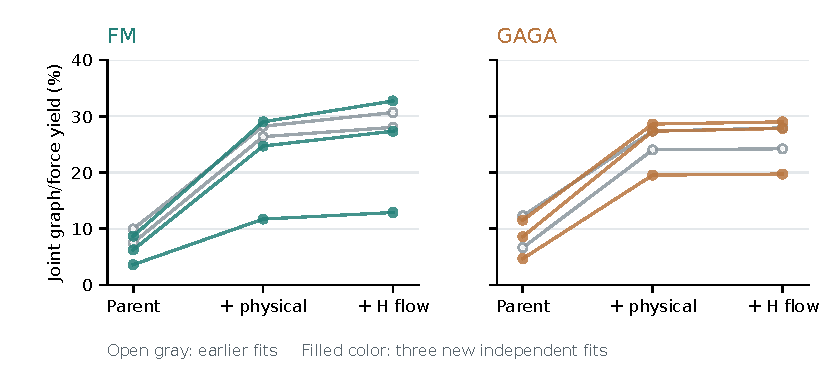
\includegraphics[width=\linewidth]{../research/figures/seed_replication_v1/five_fit_replication.pdf}

\caption{Every fitted model in the replication study. Each line follows one fixed parent through physical correction and the hydrogen readout. Gray open markers identify earlier fits; filled markers identify the three new fits. The models are compared on identical compositions and all attempts remain in the denominator.}\label{fig:seed-replication}\end{figure}

For the three new FM fits, the H flow changes all-output energy by -19.31 meV/atom relative to the fixed radial rule ($[-23.67,-15.17]$). This comparison isolates learned placement from a simple attachment rule.

With identical added modules, the five-fit FM-minus-GAGA difference is +0.78 graph-validity points ($[-0.86,2.46]$) and +0.59 joint-yield points ($[-1.04,2.21]$). Appendix~\ref{app:seed-replication} reports the new-fit subset, training uncertainty, size strata, radial controls, and force-threshold curves.
